Inhalt der \texttt{main.tex} Datei.

\begin{verbatim}
\documentclass[12pt]{scrartcl}
    
%% PREAMBLE
    %% DUMMY TEXT
\usepackage{lipsum}

%% LANGUAGE/TYPESETTING
% Set the document language
\usepackage[ngerman]{babel}

% Input of special characters, e.g. umlauts
% load this first if using the csquotes packages
\usepackage[utf8]{inputenc}

% Glyph adjust (allows correct copying of special
% characters from the PDF file
\usepackage[T1]{fontenc}

% Enables input of quotes using " "
\usepackage[autostyle=true,german=guillemets]{csquotes}
\MakeOuterQuote{"}

% No widows (last line of paragraph on a new page)
\widowpenalty10000

% No orphans (first line of paragraph on the final line of a page)
\clubpenalty10000

%% FONTS
% Arial
\usepackage{helvet}
\renewcommand{\familydefault}{\sfdefault}

%% SPACING
% Set default interline space to 1.5 * default value
\renewcommand{\baselinestretch}{1.5}

%% MARGINS
% Show page margin lines
\usepackage{showframe}
\usepackage[
    top=2.5cm,
    bottom=2.5cm,
    left=2.5cm,
    right=2.5cm,
    bindingoffset=8mm,
    ]{geometry}

    %% FORMATTING
\newcommand{\hsc}[1]{{\small\MakeUppercase{#1}}}
\newcommand{\eqn}[1]{(\ref{#1})}


%% MAIN DOCUMENT
\begin{document}
    %% Front matter
    \pagenumbering{roman}
    % Remove header, footer
\thispagestyle{empty}

\begin{flushright}
    
\includegraphics[height=2cm]{logo1}
    ~
    
\includegraphics[height=2cm]{logo2}

    \vfill

    \begin{Huge}
    Titel der Studienarbeit
    \end{Huge}

    \vspace{20pt}

    \begin{Large}
    ggf. Untertitel
    \end{Large}

    \vspace{5cm}

    \textbf{T. S.}\\
    ~\\
    weitere Angaben.\\
    ~\\
    Stand \today.

    \vspace{3cm}
\end{flushright}

    \cleardoublepage
\thispagestyle{empty}

\addsec{Danksagung}
Danke!
    
    \addsec{Abbildungsverzeichnis}
\makeatletter
\@starttoc{lof}% Print List of Figures
\makeatother
~\\


\addsec{Tabellenverzeichnis}
\makeatletter
\@starttoc{lot}% Print List of Tables
\makeatother
~\\	


%\addsec{List of symbols and abbreviations}
%~\\
%\input{./inhalt/abbrv}
	
    \tableofcontents
	
    %% Main matter
    \clearpage
    \pagenumbering{arabic}
    \section{Organisation}
\label{ch:organisation}

	\subsection{Arbeitsverzeichnis}
	\begin{figure}[H]
	\centering
	
\includegraphics[scale=1]{ordner}
	\caption{Beispiel für Datenorganisation}
\end{figure}

Je nach Editor und Kompilierungseinstellungen
kann es vorkommen, dass ein \texttt{build} Ordner
erstellt wird, in dem die temporären Dateien 
(\texttt{.aux, .log}, usw.) sich befinden.
So sieht das Arbeitsverzeichnis sauberer aus!

	
	\subsection{Dokumentenaufbau}
	Inhalt der \texttt{main.tex} Datei.

\begin{verbatim}
\documentclass[12pt]{scrartcl}
    
%% PREAMBLE
    %% DUMMY TEXT
\usepackage{lipsum}

%% LANGUAGE/TYPESETTING
% Set the document language
\usepackage[ngerman]{babel}

% Input of special characters, e.g. umlauts
% load this first if using the csquotes packages
\usepackage[utf8]{inputenc}

% Glyph adjust (allows correct copying of special
% characters from the PDF file
\usepackage[T1]{fontenc}

% Enables input of quotes using " "
\usepackage[autostyle=true,german=guillemets]{csquotes}
\MakeOuterQuote{"}

% No widows (last line of paragraph on a new page)
\widowpenalty10000

% No orphans (first line of paragraph on the final line of a page)
\clubpenalty10000

%% FONTS
% Arial
\usepackage{helvet}
\renewcommand{\familydefault}{\sfdefault}

%% SPACING
% Set default interline space to 1.5 * default value
\renewcommand{\baselinestretch}{1.5}

%% MARGINS
% Show page margin lines
\usepackage{showframe}
\usepackage[
    top=2.5cm,
    bottom=2.5cm,
    left=2.5cm,
    right=2.5cm,
    bindingoffset=8mm,
    ]{geometry}

    %% FORMATTING
\newcommand{\hsc}[1]{{\small\MakeUppercase{#1}}}
\newcommand{\eqn}[1]{(\ref{#1})}


%% MAIN DOCUMENT
\begin{document}
    %% Front matter
    \pagenumbering{roman}
    % Remove header, footer
\thispagestyle{empty}

\begin{flushright}
    
\includegraphics[height=2cm]{logo1}
    ~
    
\includegraphics[height=2cm]{logo2}

    \vfill

    \begin{Huge}
    Titel der Studienarbeit
    \end{Huge}

    \vspace{20pt}

    \begin{Large}
    ggf. Untertitel
    \end{Large}

    \vspace{5cm}

    \textbf{T. S.}\\
    ~\\
    weitere Angaben.\\
    ~\\
    Stand \today.

    \vspace{3cm}
\end{flushright}

    \cleardoublepage
\thispagestyle{empty}

\addsec{Danksagung}
Danke!
    
    \addsec{Abbildungsverzeichnis}
\makeatletter
\@starttoc{lof}% Print List of Figures
\makeatother
~\\


\addsec{Tabellenverzeichnis}
\makeatletter
\@starttoc{lot}% Print List of Tables
\makeatother
~\\	


%\addsec{List of symbols and abbreviations}
%~\\
%\input{./inhalt/abbrv}
	
    \tableofcontents
	
    %% Main matter
    \clearpage
    \pagenumbering{arabic}
    \section{Organisation}
\label{ch:organisation}

	\subsection{Arbeitsverzeichnis}
	\input{./inhalt/folder}
	
	\subsection{Dokumentenaufbau}
	\input{./inhalt/doc-structure}

	
\clearpage
\section{Front matter}
	\subsection{Deckblatt}
	\input{./inhalt/deckblatt}
	
	\subsection{Verzeichnisse}
	\input{./inhalt/verzeichnisse}

\clearpage
\section{Beispiele}
\input{./inhalt/beispiele}


\clearpage
\section{Back matter}
	Alles was nach dem Inhalt kommt, z.B.
	Quellenverzeichnis, Anhang, Index.
	
	\subsection{Bibliographie}
	\input{./inhalt/bib}
	
	\subsection{Anhang}
	\input{./inhalt/anhang}
    
    %% Back matter
    \addsec{Quellen}
%\nocite{*}						% prints uncited works
\printbibliography[heading=none]
    \addsec{Anhang}
\setcounter{subsection}{0}
\renewcommand\thesubsection{A\the\value{subsection}}

\subsection{Technical specifications of the reference sensor}
	\label{ch:appendix ati}
	~\vfill
	\begin{minipage}{\textwidth}
	\centering
	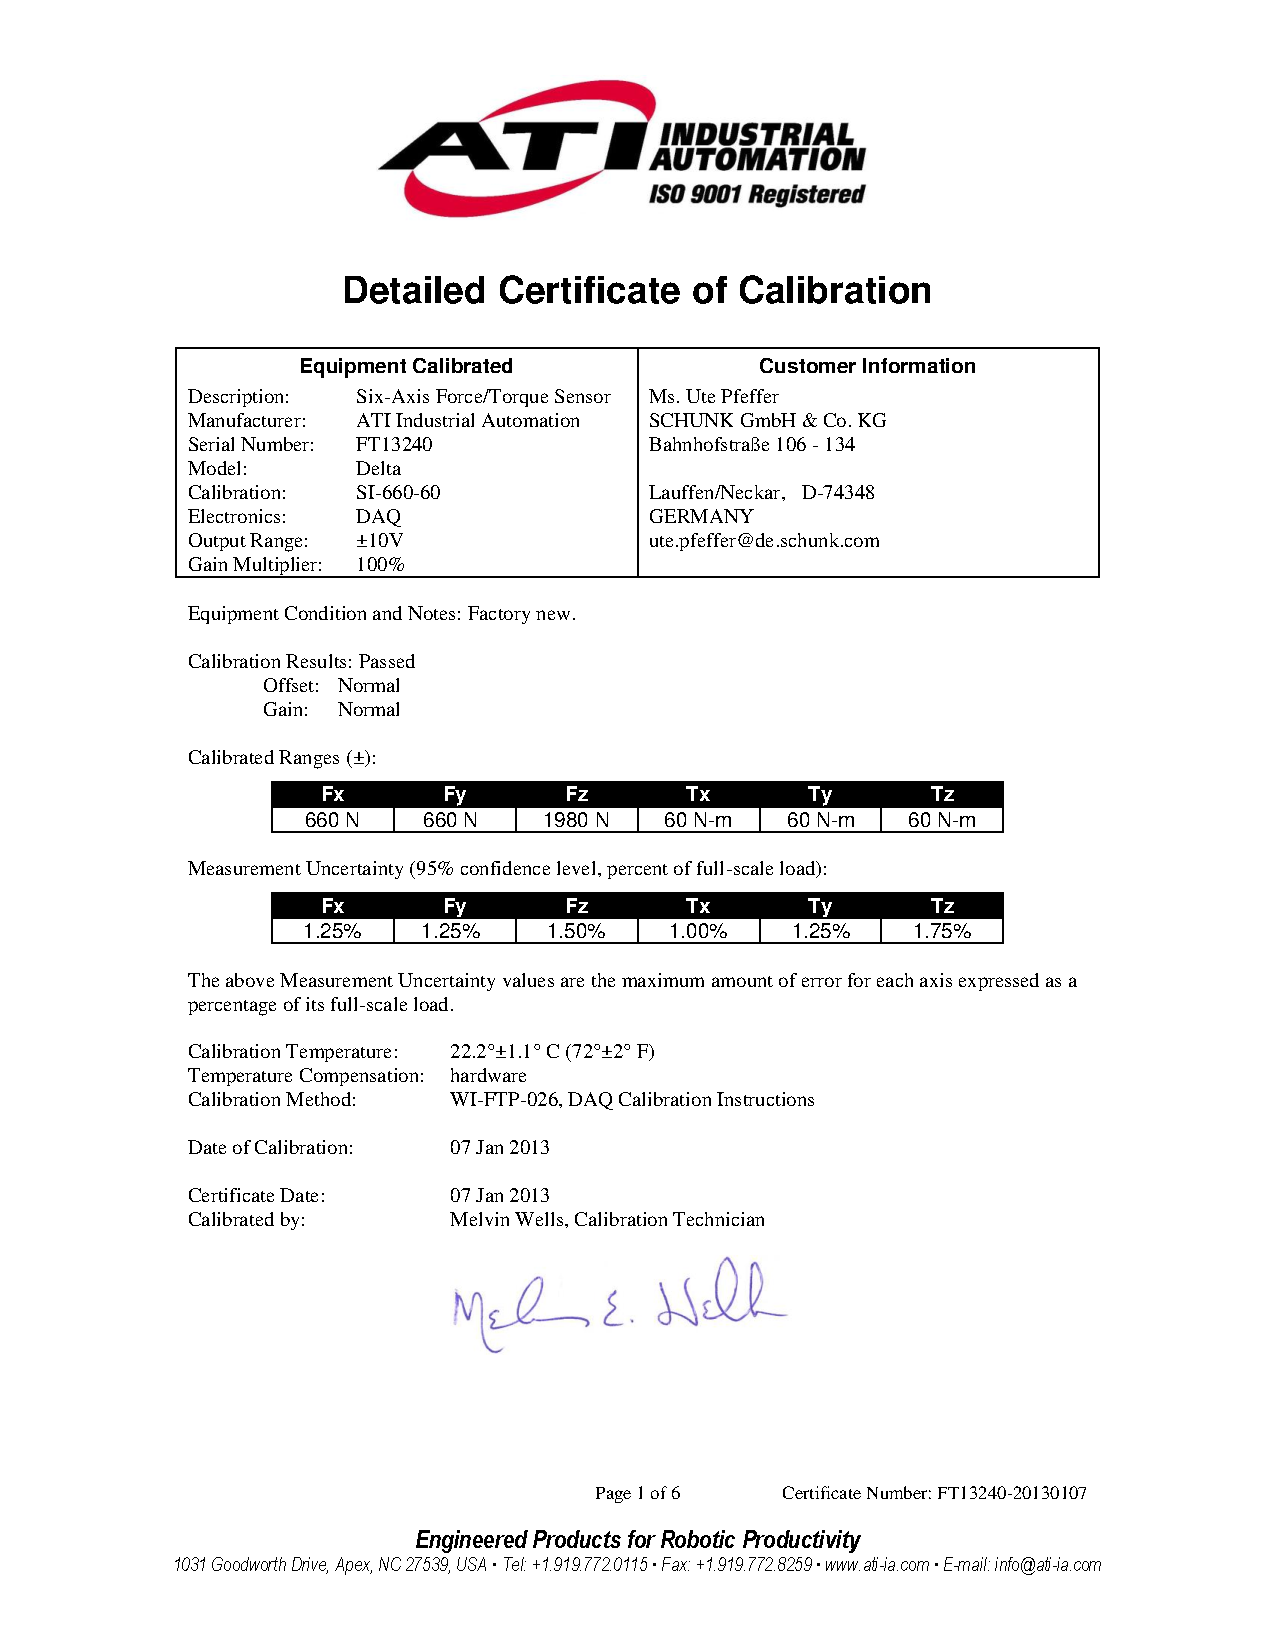
\includegraphics[scale=0.7,clip,trim=2.5cm 1cm 1cm 1cm]{atiblatt}
	\end{minipage}
	\vfill
	
\clearpage
\subsection{Script-based calculation of the calibration matrix}
	Beispieltext.
\end{document}
\end{verbatim}

Es gibt noch andere Dokumentarten
(\texttt{memoir, article, book}, usw.)
als die KOMA-Dokumentarten
(\texttt{scrartcl, scrbook}, usw.), aber die KOMA-Formate
eignen sich gut für Arbeiten,
die im deutschsprachigen Raum zu verfassen sind.\\

In  den eckigen Klammern in
\verb|\documentclass[12pt]{scrartcl}|
kann man
unter anderem die Schriftgröße des Dokuments einstellen.
Es gibt andere tolle Optionen—z.B. kann man das Dokument
auf beidseitigem Druck einstellen, indem \LaTeX{} automatisch
leere Seiten hinzufügt.
Für die anderen verfügbaren Optionen verweise ich auf
die KOMA-Dokumentation \cite{online:koma}!\\

Um externe \texttt{.tex} Dateien einzulesen, bieten sich die folgenden
Befehle an:
\begin{table}[H]
	\centering
	\begin{tabu} to \textwidth{>{\ttfamily\bfseries}ll}
	input	& Inhalte der Datei werden direkt eingelesen,
				fortgesetzt auf der aktuellen Seite.\\
	include	& Inhalte der Datei werden auf einer neuen Seite eingelesen
	\end{tabu}
\end{table}

\subsubsection{Preamble}
In der Präambel werden Pakete geladen und Stileinstellungen
festgelegt.
Ich habe in der \texttt{preamble.tex} Datei meiner Meinung nach
alles ausführlich kommentiert.\\

Man kann auch hier eigene Kommandos definieren
(hier habe ich meine Kommandos in \texttt{macros.tex} geschrieben).


\subsubsection{Hauptteil des Dokuments}
Eine akademische Ausarbeitung kann man normalerweise in drei Teilen
aufspalten:
\begin{center}
	\begin{tabu} to \textwidth{*ll}
	Front matter & Deckblatt, Danksagung, Inhaltsverzeichnis ...\\
	Main matter  & Inhaltliches\\
	Back matter  & Quellenverzeichnis, Anhang, ...
	\end{tabu}
\end{center}

Ist nicht immer fest im Stein. Manche Autoren tun ihre 
Tabellen- und Abbildungsverzeichnisse ganz hinten rein.\\

Der Front Matter hat üblicherweise römische (i, ii, ...) Seitenzahlen.
Ab dem ersten Kapitel werden arabische Zahlen (1, 2, ...)
verwendet. Daher:
\begin{verbatim}
%% Front matter
\pagenumbering{roman}
...

%% Main matter
\pagenumbering{arabic}
...
\end{verbatim}

	
\clearpage
\section{Front matter}
	\subsection{Deckblatt}
	Habe hier zwei Varianten zur Verfügung gestellt:
eine zentrierte Version, und eine rechts-ausgerichtete Version.

\begin{figure}[H]
	\centering
	\begin{subfigure}{0.45\textwidth}
		\centering
		\fbox{
\includegraphics[height=8cm]{cover1}}
		\caption{Zentrisch ausgerichtet}
	\end{subfigure}
	~
	\begin{subfigure}{0.45\textwidth}
		\centering
		\fbox{
\includegraphics[height=8cm]{cover2}}
		\caption{Rechts ausgerichtet}
	\end{subfigure}
	\caption{Deckblattvarianten}
\end{figure}

Um die Seitennummer zu entfernen:
\begin{verbatim}
\thispagestyle{empty}	
\end{verbatim}

Man kann für den Titel und Untertitel den Text in folgenden
Umgebungen umschließen:
\verb|Huge, huge, Large, large, normalsize, footnotesize, scriptsize...|	
\begin{verbatim}
\begin{Huge}
	Titel
\end{Huge}
\end{verbatim}


Rechtsausrichtung mit \verb|\begin{flushright} ... \end{flushright}|,
bzw. zentriert mit entweder \verb|\begin{center} ... \end{center}|
oder \verb|\centering|.
	
	\subsection{Verzeichnisse}
	Für die Abbildungs- und Tabellenverzeichnisse habe ich irgendwoher
mal den Code kopiert... Er ist zweiteilig:
\begin{enumerate}
	\item Formatierung in der Präambel
	\item Eigentliche Platzierung vor dem Inhaltsverzeichnis
\end{enumerate}~

In der Präambel:
\begin{verbatim}
\usepackage[titles]{tocloft}
\newlength{\figlength}
\renewcommand{\cftfigpresnum}{\figurename\enspace}
\renewcommand{\cftfigaftersnum}{:\enspace}
\settowidth{\figlength}{\cftfigpresnum\cftfigaftersnum}
\addtolength{\cftfignumwidth}{\figlength}

\newlength{\tablength}
\renewcommand{\cfttabpresnum}{\tablename\enspace}
\renewcommand{\cfttabaftersnum}{:}
\settowidth{\tablength}{\cfttabpresnum\cfttabaftersnum}
\addtolength{\cfttabnumwidth}{\tablength}
\end{verbatim}

Im Dokumententeil (\texttt{listof.tex}):
\begin{verbatim}
\addsec{Abbildungsverzeichnis}
\makeatletter
\@starttoc{lof}% Print List of Figures
\makeatother
\end{verbatim}

\clearpage
\section{Beispiele}
\subsection{Beispieltext mit Fußnote}
In diesem Abschnitt wird die nichtparametrische Systemidentifikation
eingeführt.
Es folgt die Motivation zur Berechnung im Frequenzbereich,
insbesondere mittels der Fast-Fourier-Trans\-formation.
Eine Annäherung von den Sinus-Signalen mithilfe
der Curve Fitting Methode wird ebenfalls vorgestellt%
\footnote{Dies ist eine Fußnote!}.

\begin{verbatim}
... ebenfalls vorgestellt%
\footnote{Dies ist eine Fußnote!}.
\end{verbatim}

Schreibt man \verb|\footnote{...}| 
auf einer neuen Zeile im Editor, wird im Text nach dem
letzten Wort ein Leerzeichen erstellt.
Um dies zu vermeiden, kann man am Ende der vorherigen Zeile
\% hinschreiben.
Dies unterdruckt jegliche ``whitespace character''
bis zum Anfang der nächsten Zeile.\\

\subsection{Listen}
\begin{itemize}
\item Item1
\item Item2
\end{itemize}~

\begin{enumerate}
\item Item1
\item Item2
\end{enumerate}~

\begin{verbatim}
\begin{itemize}
\item Item1
\item Item2
\end{itemize}

\begin{enumerate}
\item Item1
\item Item2
\end{enumerate}
\end{verbatim}

Es gibt ein Paar Vorformatierungen die man in der Präambel durchführen kann, z.B. mithilfe des Pakets \texttt{enumitem}.
\begin{verbatim}
\usepackage{enumitem}
\setlist{nolistsep}    % no spacing between list items
\setlist[enumerate,1]
		% list indentation
		{labelindent=0.5cm,leftmargin=*}
\end{verbatim}

\subsection{Zitationen, Verweise}
Hier mal eine Beispielzitation \cite{online:uppsala}.
\begin{verbatim}
Hier mal eine Beispielzitation \cite{online:uppsala}.\\
\end{verbatim}~

Und ein Verweis auf Kapitel \ref{ch:organisation}.
	\begin{verbatim}
	\section{Organisation}
	\label{ch:organisation}
	    ...
	
	\section{Beispiele}
	    ....
	    Und ein Verweis auf Kapitel \ref{ch:organisation}.
	\end{verbatim}~

\subsection{Formeln}
Mathematische Formeln oder Gleichungen können auch 
mitten im Absatz auftachen, z.B. $\sum_{n=1}^\infty a^i = \infty$,
wenn die Gleichung von den Zeichen \verb|$ ... $|
umgeben ist.

\begin{verbatim}
auftauchen, z.B. $\sum_{n=1}^\infty a^i = \infty$, wenn die ...
\end{verbatim}~ 

Auf einer neuen Zeile können die Gleichungen
von einer mathematischen Umgebungen umgeben werden.\\

Formel mit Nummerierung \verb|\begin{align} ... \end{align}| (Gleichung \ref{eq:formula})
\begin{align}
\int_{-\infty}^{+\infty} e^{-x^2} dx = \left( 6 \sum_{n=1}^{\infty} \frac{1}{n^2} \right)^\frac{1}{4}
\label{eq:formula}
\end{align}~

Formel ohne Nummerierung \verb|\begin{align*} ... \end{align*}|
\begin{align*}
\int_{-\infty}^{+\infty} e^{-x^2} dx = \left( 6 \sum_{n=1}^{\infty} \frac{1}{n^2} \right)^\frac{1}{4}
\end{align*}~

Formeln sind auch mithilfe der default Umgebung \verb|equation| realisierbar.
Allerdings bevorzuge ich \texttt{align}, besonders bei
mehrzeiligen Gleichungen. In \texttt{align} lassen sich nämlich
die Zeilen an dem \texttt{=} Zeichen besser ausrichten.
\begin{verbatim}
\begin{align*}
    1 + 1  &= 2\\
    341151 + 3262424 &= 3
\end{align*}
\end{verbatim}
\begin{align*}
1 + 1 &= 2\\
341151 + 3262424 &= 3
\end{align*}

\subsection{Abbildungen}
Hier sieht man ein Beispielbild
(Abbildung \ref{fig:bsp1}).

\begin{verbatim}
... Beispielbild (Abbildung \ref{fig:bsp1}).

\begin{figure}[H]
    \centering
    
\includegraphics[width=0.6\textwidth]{unilogo}
    \caption{Beispielabbildung}
    \label{fig:bsp1}
\end{figure}
\end{verbatim}

% [H] tells LaTeX to put the figure here,
% if not, LaTeX may push the figure to a 'more optimal' location
\begin{figure}[H]
\centering

\includegraphics[width=0.6\textwidth]{unilogo}
\caption{Beispielabbildung}
\label{fig:bsp1}
\end{figure}

\subsection{Tabellen}
Basic Tabellenaufbau mit dem \texttt{tabu}-Paket.
Eine Beispieltabelle ist in Tabelle \ref{tab:fit-table} zu finden.
\texttt{c} bedeutet, dass der Text in der Spalte zentriert ist.
Alternativ kann man stattdessen \texttt{l} oder \texttt{r} schreiben
(für Links- bzw. Rechtsausrichtung).

\begin{verbatim}
... ist in Tabelle \ref{tab:labelname} zu finden. ...\\

\begin{table}[H]
    \caption{Tabelle basic}
    \label{tab:labelname}
    \centering
    \begin{tabu} to \textwidth{cccc}
        \toprule
        Col1 & Col2 & Col3 & Col4\\
        \midrule
        1 & 2 & 3 & 4\\
        5 & 6 & 7 & 8\\
        \bottomrule
    \end{tabu}
\end{table}
\end{verbatim}

\begin{table}[H]
	\caption{Tabelle basic}
	\label{tab:fit-table}
	\centering
	\begin{tabu} to \textwidth{cccc}
		\toprule
		Col1 & Col2 & Col3 & Col4\\
		\midrule
		1 & 2 & 3 & 4\\
		5 & 6 & 7 & 8\\
		\bottomrule
	\end{tabu}
\end{table}~



Die obigen Tabelle \ref{tab:fit-table} hat Spaltenbreiten,
die dem Inhalt angepasst sind.
Um mehr Kontrolle über die Spaltenbreite zu haben, kann man 
die sogenannten X-columns verwenden.
Die folgende Tabelle \ref{tab:fullw-table} hat 
gleichmäßig-verteilte Spalten über die gesamte Textfeldbreite.

\begin{verbatim}
\begin{tabu} to \textwidth{X[c] X[c] X[c] X[c]}
    ....
\end{table}
\end{verbatim}

\begin{table}[H]
	\caption{Tabelle über voller Textlänge}
	\label{tab:fullw-table}
	\centering
	\begin{tabu} to \textwidth{X[c] X[c] X[c] X[c]}
		\toprule
		Col1 & Col2 & Col3 & Col4\\
		\midrule
		1 & 2 & 3 & 4\\
		5 & 6 & 7 & 8\\
		\bottomrule
	\end{tabu}
\end{table}~



Die Angabe \verb|\textwidth| kann auch z.B. zu \verb|0.6\textwidth|
umgeschrieben werden, um die Tabellenbreite zu beschränken.

\begin{verbatim}
\begin{tabu} to 0.6\textwidth{X[r] X[r] X[r] X[r]}
     ...
\end{verbatim}

\begin{table}[H]
	\caption{Tabelle über 60\% Textlänge}
	\label{tab:partial-table}
	\centering
	\begin{tabu} to 0.6\textwidth{X[r] X[r] X[r] X[r]}
		\toprule
		Col1 & Col2 & Col3 & Col4\\
		\midrule
		1 & 2 & 3 & 4\\
		5 & 6 & 7 & 8\\
		\bottomrule
	\end{tabu}
\end{table}~



Bisher hatten die Spalten alle die gleiche Breite.
Um z.B. die Breiten im Verhältnis 3:3:1:1 darzustellen, verwende
\begin{verbatim}
\begin{tabu} to 0.6\textwidth{X[3c] X[3c] X[1c] X[1c]}
    ...
\end{verbatim}

\begin{table}[H]
	\caption{Tabelle mit variablen Spaltenbreite}
	\label{tab:var-colw-table}
	\centering
	\begin{tabu} to 0.6\textwidth{X[3c] X[3c] X[1c] X[1c]}
		\toprule
		Col1 & Col2 & Col3 & Col4\\
		\midrule
		1 & 2 & 3 & 4\\
		5 & 6 & 7 & 8\\
		\bottomrule
	\end{tabu}
\end{table}~



\begin{verbatim}
\begin{tabu} to \textwidth{+l^r^r^r}
    \rowstyle{\bfseries}
    % Inhalt der ersten Zeile
    Col1 & Col2 & Col3 & Col4\\
    ...
\end{verbatim}

\begin{table}[H]
	\caption{Tabelle mit fetten Überschriften (Zeile)}
	\label{tab:bold-table-row}
	\centering
	\begin{tabu} to \textwidth{+l^r^r^r}
		\toprule
		\rowstyle{\bfseries}
		Col1 & Col2 & Col3 & Col4\\
		\midrule
		1 & 2 & 3 & 4\\
		5 & 6 & 7 & 8\\
		\bottomrule
	\end{tabu}
\end{table}~



\begin{verbatim}
\begin{tabu} to \textwidth{*l|rrr}
    ...
\end{verbatim}


\begin{table}[H]
	\caption{Tabelle mit fetten Überschriften (Spalte)}
	\label{tab:bold-table-col}
	\centering
	\begin{tabu} to \textwidth{*l|rrr}
		H1 & 11 & 21 & 31\\
		H2 & 2 & 3 & 4\\
		H3 & 6 & 7 & 8\\
	\end{tabu}
\end{table}



\clearpage
\section{Back matter}
	Alles was nach dem Inhalt kommt, z.B.
	Quellenverzeichnis, Anhang, Index.
	
	\subsection{Bibliographie}
	\subsubsection{Einstellungen in der Präambel}
Um die Literaturverzeichnis zu erstellen, muss man in der Präambel
das Paket \texttt{biblatex} laden.
Dazu sind die folgenden Optionen empfohlen.
Ansonsten kann man in die \texttt{biblatex} Dokumentation
anschauen.

\begin{verbatim}
\usepackage[backend=biber,
    sorting=nty,
    date=year,
    sortcites=true,
    ]{biblatex}
\end{verbatim}

\begin{center}
\begin{tabu} to \textwidth{>{\ttfamily}X[l] X[4l]}
	\toprule
	sorting=nty	& sorts entries by name, title, year\\
	date=year	& nur das Veröffentlichungsjahr wird gezeigt, und
		nicht das vollständige Datum\\
	sortcites=true	& obige \texttt{nty} Option wird umgesetzt\\
	\bottomrule
\end{tabu}
\end{center}

Die Informationen (Angaben zu Autor, Jahr, Titel, Auflage usw.)
werden in einer \texttt{.bib} Datei aufbewahrt und müssten
ebenfalls in der Präambel geladen werden.

\begin{verbatim}
\addbibresource{./preamble/ref.bib}
\end{verbatim}
	
Man kann an dieser Stelle auch den Stil der Bibliographie einstellen.
Z.B. nach APA, MLA, usw.
\begin{verbatim}
% Original:
% $Id: standard.bbx,v 1.6 2011/07/29 19:21:28 lehman stable $
% Angepasst:
% din.bbx, v2012-06-27, Michael Domhardt
% gekürzt nach Vorschlag von moewew vom 5. Nov. 2015, siehe: https://github.com/domhardt/BibLaTeX-DIN1505/issues/1#issuecomment-154122346


%\setlength{\bibinitsep}{\baselineskip}						% Dist. bw unlike initials
\setlength\bibhang{1em}

\DeclareNameAlias{default}{family-given}					% Last name, First name in bib
\renewcommand*{\mkbibnamefamily}[1]{\hsc{#1}}				% Small caps for last name
\renewcommand*{\multinamedelim}{\mbox{ }\addspace\addsemicolon\space}	% Semicolon b/w authors
\renewcommand*{\finalnamedelim}{\multinamedelim}			% Semicolon before last author
\renewcommand{\labelnamepunct}{\addcolon\space}				% Colon after last author
\renewcommand*{\finentrypunct}{}							% No dot at the end

\DeclareFieldFormat[inbook]{title}{#1\midsentence}			% No quote marks in chap title
\DeclareFieldFormat[inproceedings]{title}{#1\midsentence}	% No quote marks in the title
\DeclareFieldFormat{editortype}{\mkbibparens{#1}}			% Parentheses editor
\DeclareFieldFormat[thesis]{title}{\mkbibemph{#1}\midsentence}

\DefineBibliographyStrings{german}
							{urlseen = {Zugriff am}}
							
\defbibenvironment{bibliography}
	{\list{\printtext[labelnumberwidth]%
					{\printfield{labelnumber}}}
			{\setlength{\leftmargin}{\bibhang}%
			\setlength{\itemindent}{-\leftmargin}%
%			\setlength{\labelsep}{\biblabelsep}%
			\addtolength{\leftmargin}{1.75em}%
%			\setlength{\itemsep}{\bibitemsep}%
			\setlength{\parsep}{\bibparsep}
			}
	}
	{\endlist}
{\item}

% Removes comma before (Hrsg.)
\renewbibmacro*{editor+others}{%
  \ifboolexpr{
    test \ifuseeditor
    and
    not test {\ifnameundef{editor}}
  }
    {\printnames{editor}%
     \setunit{\space}% <- hier
     \usebibmacro{editor+othersstrg}%
     \clearname{editor}}
    {}}


% Defines new macro which issues \setunit to generate line breaks only (for URLs)
\newbibmacro*{bbx:parunit}{%
  \ifbibliography
    {\setunit{\bibpagerefpunct}\newblock
     \usebibmacro{pageref}%
     \clearlist{pageref}%
     \setunit{\adddot\par\nobreak}}
    {}}

% With previous code, sets URL on a new line
\renewbibmacro*{url+urldate}{%
  \usebibmacro{bbx:parunit}% Added
  \printfield{url}%
  \iffieldundef{urlyear}
    {}
    {\usebibmacro{bbx:parunit}%
     \printtext[]{\printurldate}}}

    
\DeclareBibliographyDriver{book}{% 
   \usebibmacro{bibindex}% 
   \usebibmacro{begentry}% 
   \usebibmacro{author/editor+others/translator+others}% 
		\setunit{\labelnamepunct}
   \newblock 
   \usebibmacro{maintitle+title}% 
		\newunit 
   		\printlist{language}% 
   		\newunit
   \newblock 
   \usebibmacro{byauthor}\newunit
   \newblock 
   \usebibmacro{editor+others}% 
   \newunit\newblock 
   \printfield{edition}% 
   \newunit 
   \iffieldundef{maintitle} 
     {\printfield{volume}% 
      \printfield{part}} 
     {}% 
   \newunit 
   \printfield{volumes}% 
   \newunit\newblock 
   \usebibmacro{series+number}% 
   \newunit\newblock 
   \printfield{note}% 
   \newunit\newblock 
   \usebibmacro{addendum+pubstate}%
   \setunit{\labelnamepunct}
   \newblock
   \usebibmacro{publisher+location+date}% 
   \newunit\newblock 
   \usebibmacro{chapter+pages}% 
   \newunit 
   \printfield{pagetotal}% 
   \newunit\newblock 
   \iftoggle{bbx:isbn} 
     {\printfield{isbn}} 
     {}% 
   \newunit\newblock 
   \usebibmacro{doi+eprint+url}% 
   \newunit\newblock 
   \usebibmacro{pageref}% 
   \usebibmacro{finentry}}

\DeclareBibliographyDriver{inbook}{%
  \usebibmacro{bibindex}%
  \usebibmacro{begentry}%
  \usebibmacro{author/translator+others}%
  \setunit{\labelnamepunct}\newblock
  \usebibmacro{title}%
  \newunit
  \printlist{language}%
  \newunit\newblock
  \usebibmacro{byauthor}%
  \newunit\newblock
  \usebibmacro{in:}%
  \usebibmacro{bybookauthor}%
  \newunit\newblock
  \usebibmacro{editor+others}% Herausgeber (Hrsg.) statt hrsg. von Herausgeber
  \setunit{\labelnamepunct}\newblock%
  \usebibmacro{maintitle+booktitle}%
  \newunit\newblock
  \printfield{edition}%
  \newunit
  \iffieldundef{maintitle}
    {\printfield{volume}%
     \printfield{part}}
    {}%
  \newunit
  \printfield{volumes}%
  \newunit\newblock
  \usebibmacro{series+number}%
  \newunit\newblock
  \printfield{note}%
  \newunit\newblock
  \usebibmacro{addendum+pubstate}%
  \setunit{\labelnamepunct}
  \newblock
  \usebibmacro{publisher+location+date}%
  \newunit\newblock
  \usebibmacro{chapter+pages}%
  \newunit\newblock
  \iftoggle{bbx:isbn}
    {\printfield{isbn}}
    {}%
  \newunit\newblock
  \usebibmacro{doi+eprint+url}%
  \newunit\newblock
  \usebibmacro{pageref}%
  \newunit\newblock
  \iftoggle{bbx:related}
    {\usebibmacro{related:init}%
     \usebibmacro{related}}
    {}%
  \usebibmacro{finentry}}

\DeclareBibliographyDriver{online}{% 
   \usebibmacro{bibindex}% 
   \usebibmacro{begentry}% 
   \usebibmacro{author/editor+others/translator+others}% 
   \setunit{\labelnamepunct}\newblock 
   \usebibmacro{title}% 
   \newunit\newblock 
   \usebibmacro{byauthor}% 
   \newunit\newblock 
   \usebibmacro{byeditor+others}% 
   \newunit 
   \printfield{note}% 
   \newunit\newblock 
   \printlist{organization}% 
   \newunit\newblock 
   \usebibmacro{date}% 
   \newunit\newblock 
   \iftoggle{bbx:eprint} 
     {\usebibmacro{eprint}} 
     {}% 
   \newunit\newblock 
   \usebibmacro{url+urldate}% 
   \setunit{\bibpagerefpunct}\newblock 
   \usebibmacro{pageref}% 
   \usebibmacro{finentry}}
   
\DeclareBibliographyDriver{inproceedings}{%
  \usebibmacro{bibindex}%
  \usebibmacro{begentry}%
  \usebibmacro{author/translator+others}%
  \setunit{\labelnamepunct}\newblock
  \textit{\usebibmacro{title}}%
  \newunit
  \printlist{language}%
  \newunit\newblock
  \usebibmacro{byauthor}%
  \newunit\newblock
  \usebibmacro{in:}%
  \usebibmacro{editor+others}%
  \setunit{\labelnamepunct}\newblock%
  \usebibmacro{maintitle+booktitle}%
  \usebibmacro{event+venue+date}%
%  \newunit\newblock
%  \newunit\newblock
%  \iffieldundef{maintitle}
%    {\printfield{volume}%
%     \printfield{part}}
%    {}%
%  \newunit
%  \printfield{volumes}%
%  \newunit\newblock
%  \usebibmacro{series+number}%
%  \newunit\newblock
%  \printfield{note}%
%  \newunit\newblock
%  \printlist{organization}%
%  \newunit
%  \usebibmacro{publisher+location+date}%
%  \newunit\newblock
%  \usebibmacro{chapter+pages}%
%  \newunit\newblock
%  \iftoggle{bbx:isbn}
%    {\printfield{isbn}}
%    {}%
%  \newunit\newblock
%  \usebibmacro{doi+eprint+url}%
%  \newunit\newblock
%  \usebibmacro{addendum+pubstate}%
%  \setunit{\bibpagerefpunct}\newblock
%  \usebibmacro{pageref}%
%  \newunit\newblock
%  \iftoggle{bbx:related}
%    {\usebibmacro{related:init}%
%     \usebibmacro{related}}
%    {}%
  \usebibmacro{finentry}}
   
% zusätzlicher Eintragstyp @standard
% geändert von @misc
\DeclareBibliographyDriver{standard}{%
   \usebibmacro{bibindex}% 
   \usebibmacro{begentry}% 
   \usebibmacro{author}% Nummer zuerst
   \setunit{\labelnamepunct}
   \newblock 
   \usebibmacro{title}%
   \newunit\newblock 
   \usebibmacro{addendum+pubstate}%
   \setunit{\labelnamepunct}
   \newblock
   \usebibmacro{publisher+location+date}%
   \setunit{\bibpagerefpunct}\newblock 
   \usebibmacro{pageref}% 
   \usebibmacro{finentry}}
\end{verbatim}


Ich habe bisher immer nach DIN 1505 zitiert
und die Bibliographie erstellt.
Der Code zum Bibliographiestil, den ich benutze,
ist ursprünglich von Michael Domhardt.

\subsubsection{Erstellung in der Hauptdatei}
\begin{verbatim}
\addsec{Quellen}
%\nocite{*}						% prints uncited works
\printbibliography[heading=none]
\end{verbatim}

\begin{center}
\begin{tabu} to \textwidth{>{\ttfamily}X[l] X[4l]}
	\toprule
	addsec\{...\}	& Kapitelbenennung ohne Nummer, wird im Inhaltsverzeichnis angezeigt\\
	nocite\{*\}		& falls unzitierte Werke auch aufgelistet werden sollen\\
	\bottomrule
\end{tabu}
\end{center}
	
	\subsection{Anhang}
	\begin{verbatim}
\addsec{Anhang}
\setcounter{subsection}{0}
\renewcommand\thesubsection{A\the\value{subsection}}
\end{verbatim}

Hier wurde manuell das Format der Kapitelüberschrift eingestellt,
da das Format, das ich will, nicht default vorhanden ist.
Ich wollte, dass ``Anhang'' unnummeriert im Inhaltsverzeichnis erscheint,
und dass die einzelnen Anhänge anhand A1, A2, ... durchnummeriert werden.

\begin{center}
\begin{tabu} to \textwidth{>{\ttfamily}X[l] X[4l]}
	\toprule
	addsec	& Kapitelüberschrift ohne Nummber, wird im Inhaltsverzeichnis angezeigt\\
	setcounter	& Setzt die Nummerierung von subsection zurück,
		sonst wird die Nummerierung vom Vorkapitel fortgesetzt.\\
	\bottomrule
\end{tabu}
\end{center}

Danach wie gewohnt die einzelnen Kapiteln erstellen.

\begin{verbatim}
\subsection{Erster Anhang}
    ...
    
\clearpage
\subsection{Zweiter Anhang}
    ...
\end{verbatim}
    
    %% Back matter
    \addsec{Quellen}
%\nocite{*}						% prints uncited works
\printbibliography[heading=none]
    \addsec{Anhang}
\setcounter{subsection}{0}
\renewcommand\thesubsection{A\the\value{subsection}}

\subsection{Technical specifications of the reference sensor}
	\label{ch:appendix ati}
	~\vfill
	\begin{minipage}{\textwidth}
	\centering
	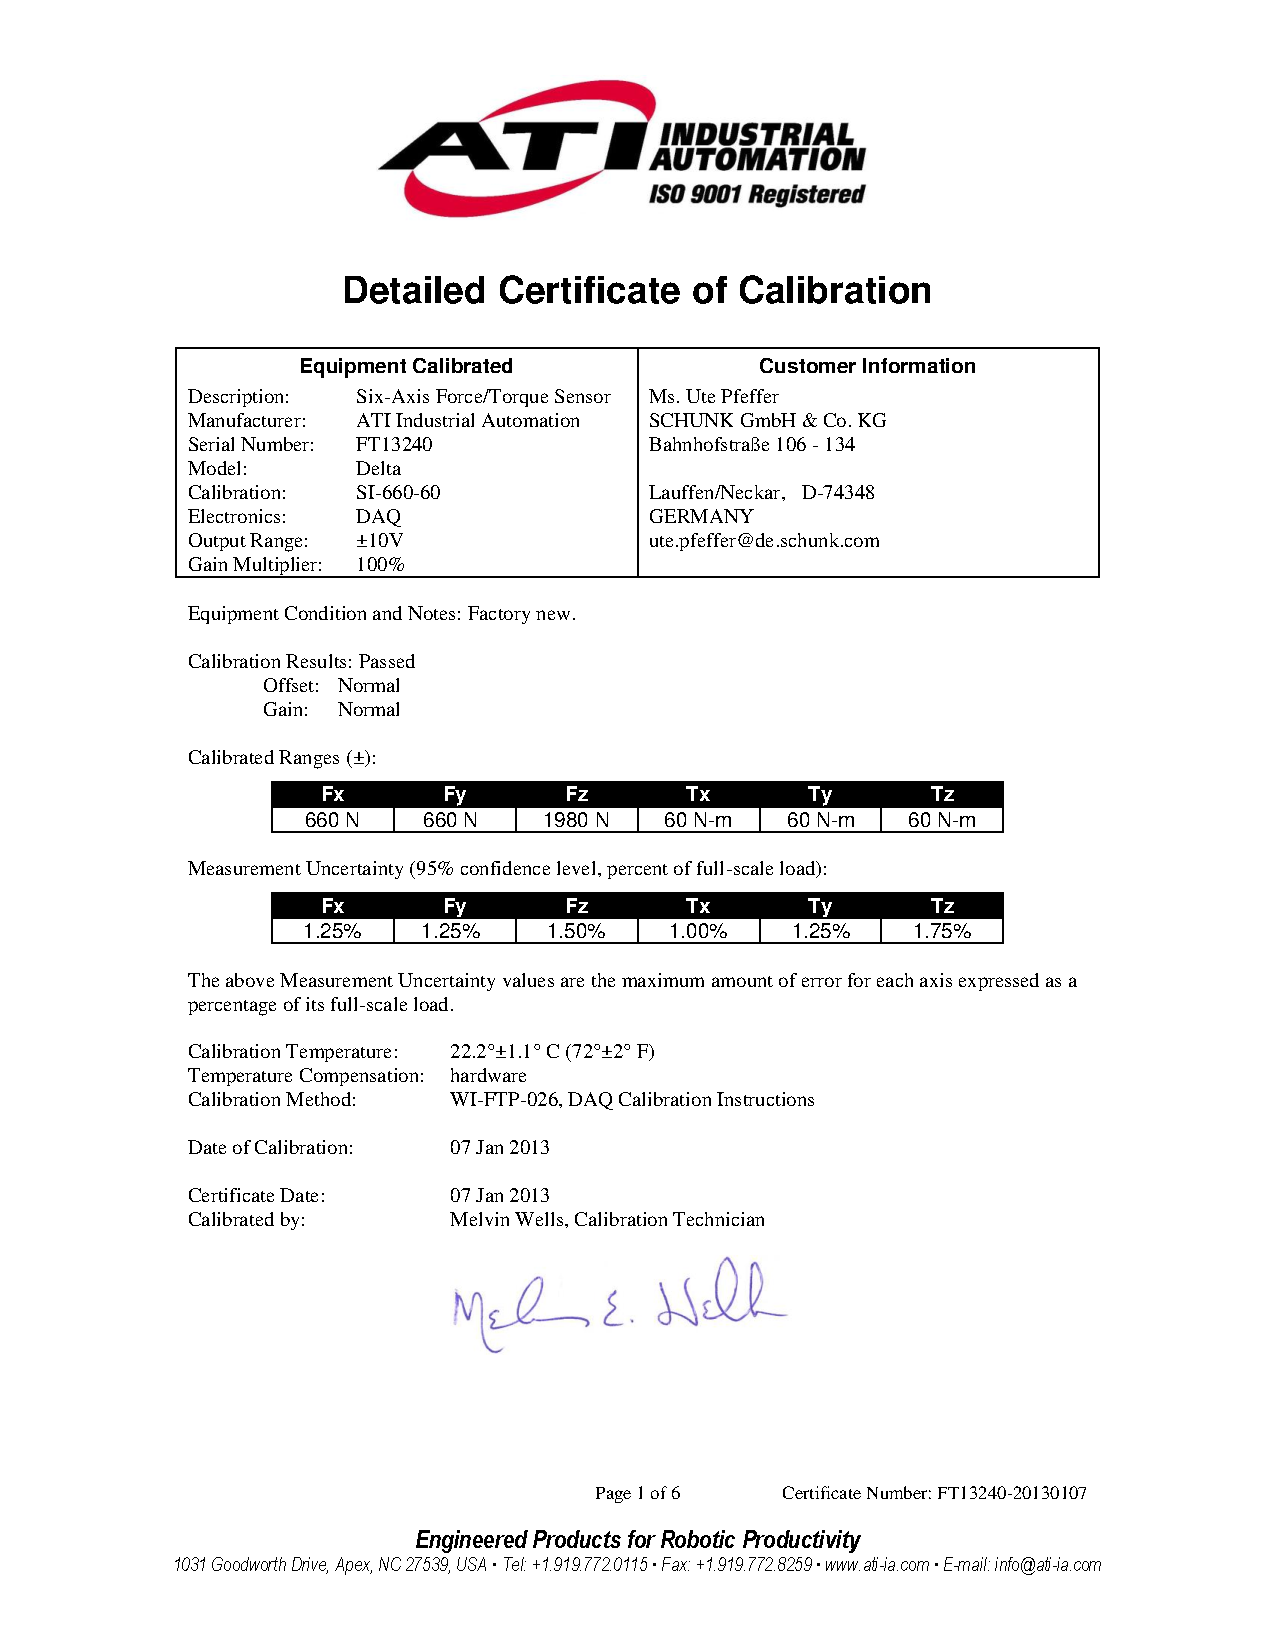
\includegraphics[scale=0.7,clip,trim=2.5cm 1cm 1cm 1cm]{atiblatt}
	\end{minipage}
	\vfill
	
\clearpage
\subsection{Script-based calculation of the calibration matrix}
	Beispieltext.
\end{document}
\end{verbatim}

Es gibt noch andere Dokumentarten
(\texttt{memoir, article, book}, usw.)
als die KOMA-Dokumentarten
(\texttt{scrartcl, scrbook}, usw.), aber die KOMA-Formate
eignen sich gut für Arbeiten,
die im deutschsprachigen Raum zu verfassen sind.\\

In  den eckigen Klammern in
\verb|\documentclass[12pt]{scrartcl}|
kann man
unter anderem die Schriftgröße des Dokuments einstellen.
Es gibt andere tolle Optionen—z.B. kann man das Dokument
auf beidseitigem Druck einstellen, indem \LaTeX{} automatisch
leere Seiten hinzufügt.
Für die anderen verfügbaren Optionen verweise ich auf
die KOMA-Dokumentation \cite{online:koma}!\\

Um externe \texttt{.tex} Dateien einzulesen, bieten sich die folgenden
Befehle an:
\begin{table}[H]
	\centering
	\begin{tabu} to \textwidth{>{\ttfamily\bfseries}ll}
	input	& Inhalte der Datei werden direkt eingelesen,
				fortgesetzt auf der aktuellen Seite.\\
	include	& Inhalte der Datei werden auf einer neuen Seite eingelesen
	\end{tabu}
\end{table}

\subsubsection{Preamble}
In der Präambel werden Pakete geladen und Stileinstellungen
festgelegt.
Ich habe in der \texttt{preamble.tex} Datei meiner Meinung nach
alles ausführlich kommentiert.\\

Man kann auch hier eigene Kommandos definieren
(hier habe ich meine Kommandos in \texttt{macros.tex} geschrieben).


\subsubsection{Hauptteil des Dokuments}
Eine akademische Ausarbeitung kann man normalerweise in drei Teilen
aufspalten:
\begin{center}
	\begin{tabu} to \textwidth{*ll}
	Front matter & Deckblatt, Danksagung, Inhaltsverzeichnis ...\\
	Main matter  & Inhaltliches\\
	Back matter  & Quellenverzeichnis, Anhang, ...
	\end{tabu}
\end{center}

Ist nicht immer fest im Stein. Manche Autoren tun ihre 
Tabellen- und Abbildungsverzeichnisse ganz hinten rein.\\

Der Front Matter hat üblicherweise römische (i, ii, ...) Seitenzahlen.
Ab dem ersten Kapitel werden arabische Zahlen (1, 2, ...)
verwendet. Daher:
\begin{verbatim}
%% Front matter
\pagenumbering{roman}
...

%% Main matter
\pagenumbering{arabic}
...
\end{verbatim}